\documentclass{beamer}

%\usepackage{lmodern}
\usepackage[font=scriptsize,skip=0pt,justification=justified,singlelinecheck=false]{caption}
%\usepackage{enumitem}
\usepackage{natbib}
\usepackage{bm}
\usepackage{mathtools}
\usepackage[makeroom]{cancel}


% Insert a Video
\usepackage{multimedia} 

% Using underline
\usepackage{soul}


%remove the icon
\setbeamertemplate{bibliography item}{}

%remove line breaks
\setbeamertemplate{bibliography entry title}{}
\setbeamertemplate{bibliography entry location}{}
\setbeamertemplate{bibliography entry note}{}
% Use number for caption
\setbeamertemplate{caption}[numbered]{}

\newtheorem{mydef}[theorem]{\Large \underline{\textbf{Definisi}}}

\makeatletter
\def\th@mystyle{%
    \normalfont % body font
    \setbeamercolor{block title example}{bg=blue,fg=white}
    \setbeamercolor{block body example}{bg=blue!20,fg=black}
    \def\inserttheoremblockenv{exampleblock}
  }
\makeatother
\theoremstyle{mystyle}
\newtheorem*{remark}{\textbf{Definition}}


% This file is a solution template for:

% - Talk at a conference/colloquium.
% - Talk length is about 20min.
% - Style is ornate.

% Copyright 2004 by Till Tantau <tantau@users.sourceforge.net>.
%
% In principle, this file can be redistributed and/or modified under
% the terms of the GNU Public License, version 2.
%
% However, this file is supposed to be a template to be modified
% for your own needs. For this reason, if you use this file as a
% template and not specifically distribute it as part of a another
% package/program, I grant the extra permission to freely copy and
% modify this file as you see fit and even to delete this copyright
% notice.  


\mode<presentation>
{
%  \usetheme{AnnArbor} % 
%	\usetheme{Frankfurt}
   \usetheme{Madrid}
%	\usetheme{Darmstadt}
  % or ...

%  \setbeamercovered{transparent}
  % or whatever (possibly just delete it)
}


\usepackage[english]{babel}
% or whatever

\usepackage[latin1]{inputenc}
% or whatever

\usepackage{times}
\usepackage[T1]{fontenc}
\usepackage{wasysym}

% Define absolute and norm
\DeclarePairedDelimiter\abs{\lvert}{\rvert}%
\DeclarePairedDelimiter\norm{\lVert}{\rVert}%

% ==============================
%       Redefine emphasize
% ==============================
\let\emph\relax % there's no \RedeclareTextFontCommand
\DeclareTextFontCommand{\emph}{\bfseries\em}


% Swap the definition of \abs* and \norm*, so that \abs
% and \norm resizes the size of the brackets, and the 
% starred version does not.
\makeatletter
\let\oldabs\abs
\def\abs{\@ifstar{\oldabs}{\oldabs*}}
%
\let\oldnorm\norm
\def\norm{\@ifstar{\oldnorm}{\oldnorm*}}
\makeatother

\usepackage{color}
\definecolor{myblue}{rgb}{.8,.8,1}
\usepackage{empheq}
% Or whatever. Note that the encoding and the font should match. If T1
% does not look nice, try deleting the line with the fontenc.

\newlength\mytemplen
\newsavebox\mytempbox

\makeatletter
\newcommand\mybluebox{%
    \@ifnextchar[%]
       {\@mybluebox}%
       {\@mybluebox[0pt]}}

\def\@mybluebox[#1]{%
    \@ifnextchar[%]
       {\@@mybluebox[#1]}%
       {\@@mybluebox[#1][0pt]}}

\def\@@mybluebox[#1][#2]#3{
    \sbox\mytempbox{#3}%
    \mytemplen\ht\mytempbox
    \advance\mytemplen #1\relax
    \ht\mytempbox\mytemplen
    \mytemplen\dp\mytempbox
    \advance\mytemplen #2\relax
    \dp\mytempbox\mytemplen
    \colorbox{myblue}{\hspace{1em}\usebox{\mytempbox}\hspace{1em}}}

\makeatother

\title[Fatherless Generasi] % (optional, use only with long paper titles)
{\textbf{Fatherless Generation}}

%\subtitle
%{\textit{Perbedaan Pria dan Wanita}}

\author[Hendra Bunyamin] % (optional, use only with lots of authors)
{Hendra Bunyamin}
%{F.~Author\inst{1} \and S.~Another\inst{2}} --> original
% - Give the names in the same order as the appear in the paper.
% - Use the \inst{?} command only if the authors have different
%   affiliation.

\institute[ ] % (optional, but mostly needed)
{
%  \inst{1}%
  \hfill \break
  \hfill \break 
  \hfill \break
  \hfill \break
  \large
  Renungan KOMIT Pria\\
  GKI Anugerah
%  \and
%  \inst{2}%
%  Department of Theoretical Philosophy\\
%  University of Elsewhere
}
% - Use the \inst command only if there are several affiliations.
% - Keep it simple, no one is interested in your street address.

%\date[CFP 2003] % (optional, should be abbreviation of conference name)
%{Conference on Fabulous Presentations, 2003}
% - Either use conference name or its abbreviation.
% - Not really informative to the audience, more for people (including
%   yourself) who are reading the slides online

\subject{PowerPoint}
% This is only inserted into the PDF information catalog. Can be left
% out. 

% If you have a file called "university-logo-filename.xxx", where xxx
% is a graphic format that can be processed by latex or pdflatex,
% resp., then you can add a logo as follows:

\pgfdeclareimage[height=1.2cm]{university-logo}{images/logo-gkia-komit}
\logo{\pgfuseimage{university-logo}}


% Delete this, if you do not want the table of contents to pop up at
% the beginning of each subsection:
\AtBeginSection[]
{
  \begin{frame}<beamer>{Outline}
    \tableofcontents[currentsection,currentsection]
  \end{frame}
}


% If you wish to uncover everything in a step-wise fashion, uncomment
% the following command: 

%\beamerdefaultoverlayspecification{<+->}

\begin{document}

\begin{frame}
  \titlepage
\end{frame}

\begin{frame}{Outline}
  \tableofcontents
  % You might wish to add the option [pausesections]
\end{frame}


% Structuring a talk is a difficult task and the following structure
% may not be suitable. Here are some rules that apply for this
% solution: 

% - Exactly two or three sections (other than the summary).
% - At *most* three subsections per section.
% - Talk about 30s to 2min per frame. So there should be between about
%   15 and 30 frames, all told.

% - A conference audience is likely to know very little of what you
%   are going to talk about. So *simplify*!
% - In a 20min talk, getting the main ideas across is hard
%   enough. Leave out details, even if it means being less precise than
%   you think necessary.
% - If you omit details that are vital to the proof/implementation,
%   just say so once. Everybody will be happy with that.

%\begin{frame}{Make Titles Informative. Use Uppercase Letters.}{Subtitles are optional.}


\section{Kehadiran \& Pengaruh Ayah}
\begin{frame}{Tabel Kehadiran-Pengaruh Ayah (1/2)}
	\begin{figure}[!ht]
		\centering
		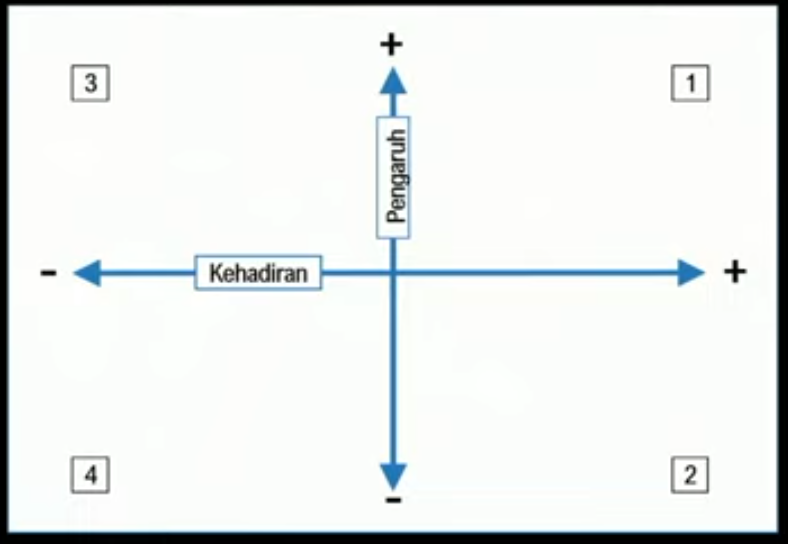
\includegraphics[scale=.3]{images/diagram-fatherless}
	\end{figure}
\end{frame}

\begin{frame}{Tabel Kehadiran-Pengaruh Ayah (2/2)}
	\begin{figure}[!ht]
		\centering
		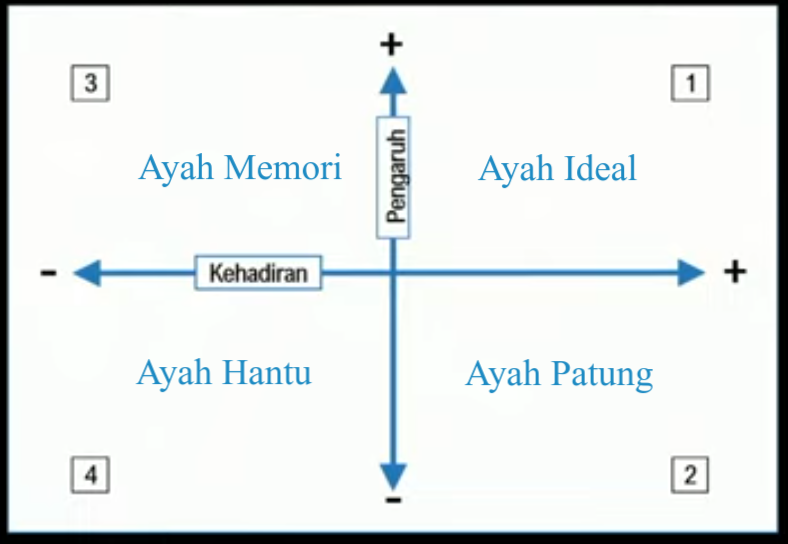
\includegraphics[scale=.3]{images/tabel-ayah-komplit}
	\end{figure}
\end{frame}

\begin{frame}{Anak Mengenal Allah ...}	
	\begin{block}{\textbf{Kejadian 1:26-27}}
	Berfirmanlah Allah: "Baiklah Kita menjadikan manusia menurut gambar dan rupa Kita, supaya mereka berkuasa atas ikan-ikan di laut dan burung-burung di udara dan atas ternak dan atas seluruh bumi dan atas segala binatang melata yang merayap di bumi." Maka \textbf{Allah menciptakan manusia itu menurut gambar-Nya}, menurut gambar Allah diciptakan-Nya dia; \textbf{laki-laki dan perempuan diciptakan-Nya mereka}. 	
	\end{block}
	
	\bigskip
	$\Longrightarrow$ anak mengenal Allah melalui ayah dan ibunya.
\end{frame}

\section{Rancangan Allah bagi Kita Semua}
\begin{frame}{Rancangan Allah bagi Ayah}	
	\begin{block}{\textbf{Kejadian 2:15-18}}
TUHAN Allah mengambil manusia itu dan menempatkannya dalam taman Eden untuk \textbf{mengusahakan dan memelihara} taman itu. Lalu TUHAN Allah memberi perintah ini kepada manusia: "Semua pohon dalam taman ini boleh kaumakan buahnya dengan bebas, tetapi pohon pengetahuan tentang yang baik dan yang jahat itu, janganlah kaumakan buahnya, sebab pada hari engkau memakannya, pastilah engkau mati. "TUHAN Allah berfirman: "Tidak baik, kalau manusia itu seorang diri saja. Aku akan menjadikan \textbf{penolong} baginya, yang sepadan dengan dia."
	\end{block}
\end{frame}

\begin{frame}{Rancangan Allah (1/3)}
	\begin{itemize}
		\item Rancangan Allah adalah ayah yang \textbf{hadir dan menghadirkan Allah}.
	\end{itemize}
\end{frame}

\begin{frame}{Rancangan Allah (2/3)}
	\begin{figure}[!ht]
	\centering
	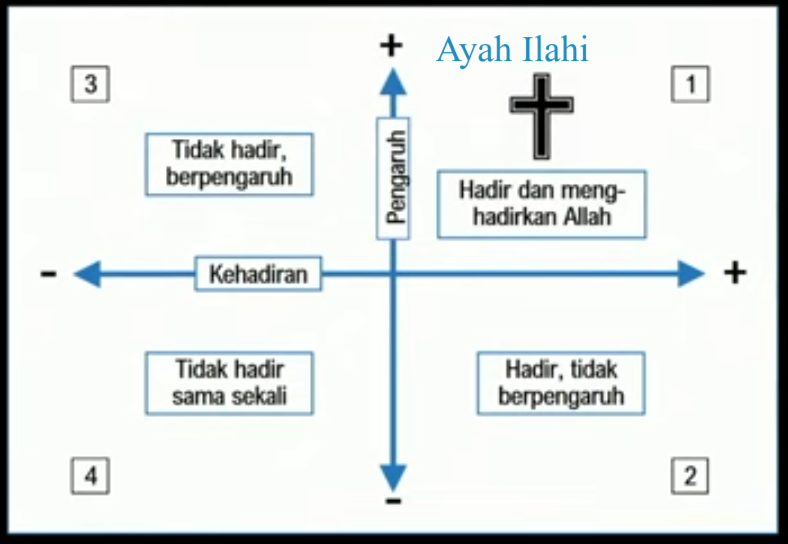
\includegraphics[scale=.3]{images/tabel-ayah-ilahi}
\end{figure}
\end{frame}

\begin{frame}{Rancangan Allah (3/3)}
	\begin{itemize}
		\item Rancangan Allah adalah ayah yang \textbf{hadir dan menghadirkan Allah}.
		\item Rancangan Ibu adalah \textbf{menolong} ayah untuk menjadi apa yang Allah rancangkan.
	\end{itemize}
\end{frame}

\begin{frame}{Ayah}
	\begin{figure}[!ht]
	\centering
	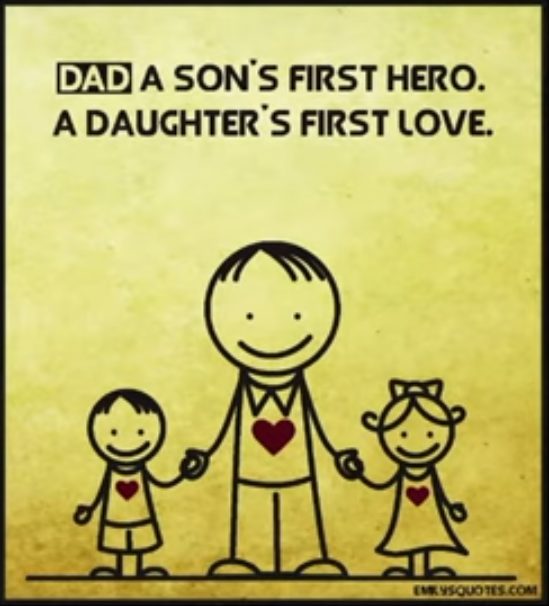
\includegraphics[scale=.3]{images/ayah-cinta-pertama}
	\caption{Ayah, pahlawan pertama bagi putranya. Cinta pertama bagi putrinya.}
\end{figure}	
\end{frame}

\section{Rancangan yang Rusak}
\begin{frame}{Rancangan yang Rusak (1/2)}
	\begin{block}{\textbf{Kejadian 3:6}}
		\textbf{Perempuan} itu melihat, bahwa buah pohon itu baik untuk dimakan dan sedap kelihatannya, lagipula pohon itu menarik hati karena memberi pengertian. Lalu ia mengambil dari buahnya dan dimakannya dan diberikannya juga kepada suaminya yang bersama-sama dengan dia, dan suaminyapun memakannya
	\end{block}

	\bigskip
	Menjadi terbalik: binatang $\longrightarrow$ Hawa $\longrightarrow$ Adam $\longrightarrow$ Tuhan.
\end{frame}

\begin{frame}{Rancangan yang Rusak (2/2)}
	\begin{itemize}
		\item Suami kurang percaya diri karena istri kurang memberi kesempatan kepada suami untuk bertumbuh.
		\item Suami kurang percaya diri karena istri kurang memberi kesempatan kepada suami untuk mengalami apa yang Allah rancangkan.
		\item Istri mengambil alih $\longrightarrow$ masalah beres dalam jangka pendek.
		\item Jangka panjang $\longrightarrow$ semakin jauh dari rancangan Tuhan.
	\end{itemize}
\end{frame}

\section{Pemulihan dalam Kristus}
\begin{frame}{Pemulihan dalam Kristus (1/2)}
	\begin{block}{\textbf{Maleakhi 4:4-6}}
		Ingatlah kepada Taurat yang telah Kuperintahkan kepada Musa, hamba-Ku, di gunung Horeb untuk disampaikan kepada seluruh Israel, yakni ketetapan-ketetapan dan hukum-hukum. Sesungguhnya Aku akan mengutus nabi Elia kepadamu menjelang datangnya hari TUHAN yang besar dan dahsyat itu. Maka ia akan membuat hati bapa-bapa berbalik kepada anak-anaknya dan hati anak-anak kepada bapa-bapanya supaya jangan Aku datang memukul bumi sehingga musnah.
	\end{block}
\end{frame}

\begin{frame}{Pemulihan dalam Kristus (2/2)}
\begin{itemize}
	\item Ayah yang \textbf{menyadari kesalahannya dan meminta maaf} kepada anak.
	\item Anak yang sekarang memiliki Bapa yang sempurna dan mengasihinya, dapat mengampuni dan menerima sang ayah.
\end{itemize}
\end{frame}

\begin{frame}{Tabel Kehadiran-Pengaruh Ayah: \textbf{Ayah Ilahi}}
	\begin{figure}[!ht]
	\centering
	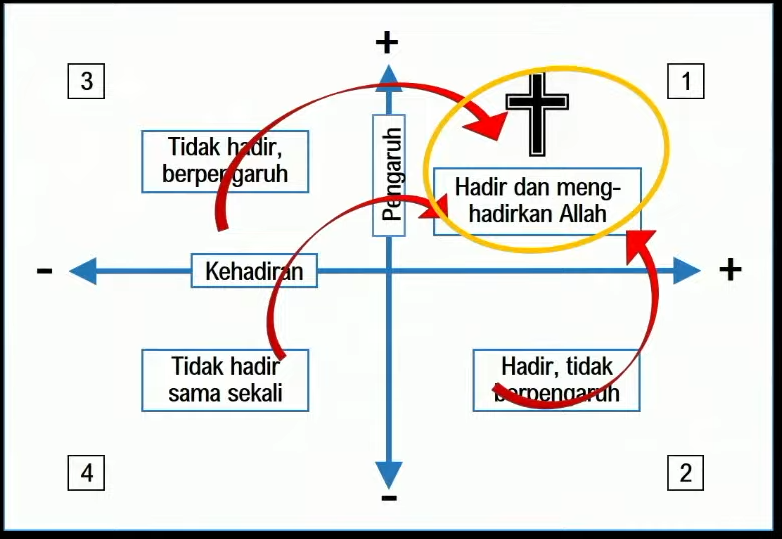
\includegraphics[scale=.3]{images/tabel-ayah-ilahi-panah}
\end{figure}	
Untuk para istri, jangan hilang pengharapan.\\ 
Pengharapan itu selalu ada sekecil apapun.
\end{frame}

\begin{frame}{Allah yang Hadir \& Menghadirkan Allah}
	\begin{table}[!ht]
		\begin{tabular}{|l|l|}
			\hline
			\textbf{Peran Ayah}           & \textbf{Dampak terhadap anak} \\
			\hline
			Kedekatan dengan Allah        & Pengajaran kepada anak \\
			\hline
			Keteladanan hidup yang benar  & Panutan untuk anak \\
			\hline
			Keintiman relasi dengan anak  & Pengalaman iman bersama anak \\
			\hline
		\end{tabular}
	\end{table}
\end{frame}

\section{Pertanyaan Refleksi}
\begin{frame}{Pertanyaan Refleksi (1/2)}
	\begin{itemize}
		\item<2-> Apakah rancangan Allah bagi keluarga, khususnya bagi seorang ayah, sudah terjadi dalam keluarga kita? Maukah kita sama-sama berusaha untuk kembali kepada rancangan Allah ini? Bila kita menyadari terjadi penyimpangan dari rancangan Allah ini, marilah kita bersama, baik suami maupun istri, belajar taat dalam hal ini.
		\item<3-> Apa yang akan kita lakukan, ketika kebenaran yang begitu gamblang dinyatakan di hadapan kita, akibat buruk dari kegagalan seorang ayah? Apakah yang akan kita lakukan untuk memperbaiki keadaan yang sedang terjadi dalam keluarga kita atau di sekeliling kita?
		\item<4-> Bagaimanakah kehadiran sosok ayah dalam keluarga kita? Ungkapkanlah dengan jujur di hadapan Tuhan, kondisi nyata dalam diri atau keluarga kita. Mulailah berusaha untuk bisa menjadi seperti yang Allah kehendaki. Mulailah dari diri sendiri dan kemudian dengan pasangan
		kita.
	\end{itemize}
\end{frame}

\begin{frame}{Pertanyaan Refleksi (2/2)}
	\begin{itemize}
		\item<2-> Bagaimanakah pemulihan relasi dalam keluarga kita? Apabila Anda rindu dan kita percaya bahwa relasi yang harmonis dalam Kristus, bisa terjadi di tengah keretakan yang terparah sekalipun, mulailah dari diri kita sendiri. Apakah yang akan kita ubah dan mulai lakukan?
		\item<3-> Bagaimanakah relasi Anda dengan ayah atau anak Anda? Apakah ada hal-hal yang perlu diperbaiki? Ataukah ada relasi yang perlu dipulihkan? Mohon pertolongan Tuhan, agar bisa menjadi sesuatu yang lebih indah dan harmonis dalam keluarga Anda. Dan mulailah dengan
		tindakan-tindakan kecil sekarang juga!
	\end{itemize}
\end{frame}
%\begin{frame}{Blocks}
%\begin{block}{Block Title}
%You can also highlight sections of your presentation in a block, with it's own title
%\end{block}
%\begin{theorem}
%There are separate environments for theorems, examples, definitions and proofs.
%\end{theorem}
%\begin{example}
%Here is an example of an example block.
%\end{example}
%\end{frame}


% All of the following is optional and typically not needed. 
%\appendix
%\section<presentation>*{\appendixname}
%\subsection<presentation>*{For Further Reading}
%
%\begin{frame}[allowframebreaks]
%  \frametitle<presentation>{Daftar Pustaka}
%    {\footnotesize
%    \bibliographystyle{apalike}
%    \bibliography{references}
%    }    
%\end{frame}

%\makeatletter % to change template
%    \setbeamertemplate{headline}[default] % not mandatory, but I though it was better to set it blank
%    \def\beamer@entrycode{\vspace*{-\headheight}} % here is the part we are interested in :)
%\makeatother

%\begin{frame}[plain]
%		\centering
\includegraphics[scale=0.5]{Logo-Maranatha-Untuk-Belakang-02}	
%\end{frame}

\begin{frame}[plain]
		\centering
\includegraphics[scale=1]{images/thank-you}	
		hendra.bunyamin@it.maranatha.edu
\end{frame}

\end{document}

